\documentclass[12pt]{amsart}
\usepackage{preamble}
\DeclareMathOperator{\stab}{\mathrm{stab}}

\usepackage{tikz-3dplot} 
\usetikzlibrary{decorations.markings}
\tikzset{->-/.style={decoration={% https://tex.stackexchange.com/a/39282/194703
  markings,
  mark=at position #1 with {\arrow{>}}},postaction={decorate}},
  ->-/.default=0.5}

\begin{document}
\begin{center}
    \textsc{Math 601. HW 6\\ Ian Jorquera}
\end{center}
\vspace{1em}
\begin{itemize} % 15 point completed
    \item[(1)] % 1 point 
    The dimension of the adjoint representation of $\mathfrak{gl}_n$ is the 
    dimension of $\mathfrak{gl}_n$ as a vector space which is $n^2$ as it is spanned by 
    the matrices $E_{ij}$ for all $i,j$.\\
    \item[(2)] % 4 points$
    Recall that $\mathfrak{k}$ are all $n\times n$ matrices. 
    First notice that the Cartan subalgebra $\mathfrak{h}$ for $\mathfrak{gl}_n$ 
    are the diagonal matrices. To see this let $H$ be any matrix and let $E_{ij}$ 
    be the elementary matrix with a $1$ is row $i$ column $j$ and zero everywhere else.
    Notice that for $[H,{E_{ij}}]$ to be a multiple of $E_{ij}$, $H$ must be diagonal.
    Let the diagonal entries be $x_1,\dots, x_n$, in which case $[H,{E_{ij}}]=(x_i-x_j)E_{ij}$.
    Notice also that diagonal matrices always commute, meaning the 
    subalgebra of diagonal matrices is abelian, showing it is the Cartan subalgebra.
    We can also fix a basis for the dial space.
    Let the function $L_i:\mathfrak{h}\ra \C$ be the map that takes a diagonal matrix
    with diagonal entries be $x_1,\dots, x_n$ and maps it to $x_i$. Notice that these span 
    the dual of the Cartan Subalgebra

    Now we will determine the roots of $\mathfrak{gl}_n$, the weights of the adjoint 
    representation. Because $\mathfrak{gl}_n$ 
    as a vector space is spanned by the elementary matrices $E_{ij}$. We can look at how the 
    Cartan subsalgebra acts on this basis, to determine the roots. From before we observed
    $[H,{E_{ij}}]=(x_i-x_j)E_{ij}=\alpha(H)E_{ij}$, where $\alpha=L_i-L_j\in\mathfrak{h}^*$.
    So the roots of $\mathfrak{gl}n$ are non-zero weights $\{L_i-L_j| i\neq j\}$.

    Notice that these are exactly the same roots as $\mathfrak{sl}_n$. We can conclude that 
    $\mathfrak{gl}_n$ is not semisimple because the roots only span the space of trace zero
    diagonal matrices which is one dimension smaller then the space of all diagonal matrices
    which is the cartan subalgebra of $\mathfrak{gl}_n$.\\
    \item[(3)] 
    We will use the definition $\mathfrak{s0}_{2n+1}=\{X\in \C^{2n+1\times 2n+1}: X^tS+SX=0\}$ where 
    \[S=\begin{bmatrix}[c|cc]
        1 &0 &0\\
        \hline
        0 &0 &I_n\\
        0 &I_n& 0
    \end{bmatrix}\]
    Notice that because $S$ is a permutation matrix $S^{-1}=S^t$ and because 
    $S$ is symmetric, $S^{-1}=S^t=S$. So we can rewrite the defining equation as $X^t=-SXS$.
    Now let $X_1,X_2,X_3,X_4\in \C^{n\times n}$, and $y_1,y_2,y_3,y_4\in \C^n$ then 
    \[X=\begin{bmatrix}[c|ccc|ccc]
        0 &&y_1^t&&&y_2^t&\\
        \hline
        &&&&&&\\
        y_3&&X_1&&&X_2&\\
        &&&&&&\\
        \hline
        &&&&&&\\
        y_3&&X_1&&&X_2&\\
        &&&&&&\\
    \end{bmatrix} X^t=\begin{bmatrix}[c|ccc|ccc]
        0 &&y_3^t&&&y_4^t&\\
        \hline
        &&&&&&\\
        y_1&&X_1^t&&&X_3^t&\\
        &&&&&&\\
        \hline
        &&&&&&\\
        y_2&&X_2^t&&&X_4^t&\\
        &&&&&&\\
    \end{bmatrix} SXS=\begin{bmatrix}[c|ccc|ccc]
        0 &&-y_2^t&&&-y_1^t&\\
        \hline
        &&&&&&\\
        -y_4&&-X_4&&&-X_3&\\
        &&&&&&\\
        \hline
        &&&&&&\\
        -y_3&&-X_2&&&-X_1&\\
        &&&&&&\\
    \end{bmatrix}\]
    Giving us $y_1=-y_4$, $y_2=-y_3$, $X_1^t=-X_4$, $X_2^t=-X_2$, $X_3^t=-X_3$ which tells 
    us about the redundant basis elements $\mathfrak{s0}_{2n+1}$. The first two equations 
    give us $2n$ basis elements, the third gives $n^2$ and the last two give $n^2-n$. All 
    combined we have $\dim(\mathfrak{s0}_{2n+1})=2n^2+n$.\\

    \item[(4)] % 3 points
    We will use the definition $\mathfrak{s0}_{5}=\{X\in \C^{5\times 5}: X^tS+SX=0\}$ where 
    \[S=\begin{bmatrix}[c|cc]
        1 &0 &0\\
        \hline
        0 &0 &I_2\\
        0 &I_2& 0
    \end{bmatrix}\]
    This along with the work from the previous problems gives us a basis 
    \begin{equation*}
        \begin{split}
        \{E_{12}-E_{41},E_{13}-E_{51}, E_{14}-E_{21}, E_{15}-E_{31},\\ % for the ys
        E_{22}-E_{44}, E_{23}-E_{54}, E_{32}-E_{45}, E_{33}-E_{55},\\ % for X_1, X_4
        E_{25}-E_{34}, E_{43}-E_{52}
        \}
        \end{split}
    \end{equation*}
    Where the first row are the basis elements determining the blocks for the $y$s, the second for 
    $X_1$ and $X_4$ and third line for $X_2$ and $X_3$. So this is the basis for the adjoint representation.
    To see how this corresponds the the adjoint representation, we need to determine the roots, 
    which means we need determine what the Cartan Subalgebra. Because of the definition 
    \[\mathfrak{h}=\{\begin{bmatrix}[c|cc|cc]
        0&0&0&0&0\\
        \hline
        0&a&0&0&0\\
        0&0&b&0&0\\
        \hline
        0&0&0&-a&0\\
        0&0&0&0&-b\\
    \end{bmatrix}\}\]
    This also means the dual of the Cartan is spanned by $L_1,L_2$ which maps diagonal 
    matrices to $a$ and $b$ respectively 
    So we can look at how this multiplies with a general matrix in $\mathfrak{so}_{2n+1}$

    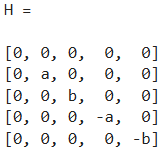
\includegraphics[width=100px]{hw6-1.png}
    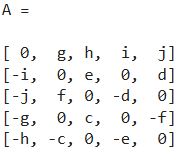
\includegraphics[width=100px]{hw6-2.png}
    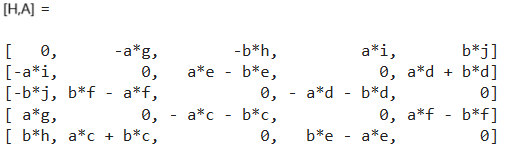
\includegraphics[width=240px]{hw6-3.png}
    
    This shows us that the Roots are $\{\pm L_1, \pm L_2, \pm L_1\pm L_2\}$ which is 
    exactly the root system for type $B$. To see this a bit more we can now that $L_1$ and $L_2$ are 
    orthogonal and span a real $2$ dimensional space, so the roots are exactly the drawing for 
    type B we already know and love.
    We also have a choice of positive simple roots being $L_1, L_2-L_1$.\\
    
    
    \item[(7)] % 3 points
    The corresponding Dynkin Diagram for $\mathfrak{sl}_4$ is 3 dots, so there are 
    $3$ unit norm simple roots, $2$ are pairwise orthogonal and all angles are $2/3\pi$. 
    We can denote them as 
    \[s_1=\begin{bmatrix}1\\0\\0\end{bmatrix},
    s_2=\begin{bmatrix}0\\1\\0\end{bmatrix},
    s_3=\begin{bmatrix}-1/2\\-1/2\\1/\sqrt{2}\end{bmatrix}\]
    And are shown in red in th diagram below.
    Next we can add in the negatives of these roots. And finally consider the 
    reflections of the simple roots where we get the following
    \[s_1+s_3=\begin{bmatrix}1/2\\-1/2\\1/\sqrt{2}\end{bmatrix},
    s_1+s_3=\begin{bmatrix}-1/2\\1/2\\1/\sqrt{2}\end{bmatrix}\]
    and there negatives. And then again we can look at the reflections of these with the simple roots and get
    \[s_1+s_2+s_3=\begin{bmatrix}1/2\\1/2\\1/\sqrt{2}\end{bmatrix}\]
    This gives us a total of $12$ roots.
    We know that the roots of $\mathfrak{sl}_4$ are $\{L_i-L_j| i\neq j\}$, meaning there are $12$ total roots,
    and so we know the root system would be the following
    
    
    \tdplotsetmaincoords{70}{125}
    \begin{tikzpicture}[tdplot_main_coords,line cap=round,>=stealth]
        \draw (-2,0,0) --  (2,0,0)  node[pos=1.05]{$x$};
        \draw (0,-2,0) -- (0,2,0) node[pos=1.05]{$y$};
        \draw (0,0,-2) -- (0,0,2) node[pos=1.05]{$z$};
        \draw (1,0,0) node[below]{$1$} -- ++ (0,0,0.15)
        (0,1,0) node[below]{$1$} -- ++ (0,0,0.15)
        (0,0,-1) node[right]{$-1$} -- ++ (0,-0.15,0)
        (0,0,1) node[right]{$1$} -- ++ (0,-0.15,0);
        % simple roots
        \draw[very thick,->=1,red] (0,0,0)  -- (1,0,0);%s_1
        \draw[very thick,->=1,red] (0,0,0)  -- (0,1,0);%s_2
        \draw[very thick,->=1,red] (0,0,0)  -- (-.5,-.5,0.7071);%s_3
        % negative of simples
        \draw[very thick,->=1] (0,0,0)  -- (-1,0,0);
        \draw[very thick,->=1] (0,0,0)  -- (0,-1,0);
        \draw[very thick,->=1] (0,0,0)  -- (.5,.5,-0.7071);
        % positive integer linear combinations of simple roots

        %Add reflections and their negatives, also linear combinations
        \draw[very thick,->=1] (0,0,0)  -- (.5,-.5,0.7071);%s_1+s_3
        \draw[very thick,->=1] (0,0,0)  -- (-.5,.5,-0.7071);
        \draw[very thick,->=1] (0,0,0)  -- (-.5,.5,0.7071);%s_2+s_3
        \draw[very thick,->=1] (0,0,0)  -- (.5,-.5,-0.7071);
        \draw[very thick,->=1] (0,0,0)  -- (.5,.5,0.7071);%s_1+s_2+s_3
        \draw[very thick,->=1] (0,0,0)  -- (-.5,-.5,-0.7071);
    \end{tikzpicture}
    \tdplotsetmaincoords{70}{-125}
    \begin{tikzpicture}[tdplot_main_coords,line cap=round,>=stealth]
        \draw (-2,0,0) --  (2,0,0)  node[pos=1.05]{$x$};
        \draw (0,-2,0) -- (0,2,0) node[pos=1.05]{$y$};
        \draw (0,0,-2) -- (0,0,2) node[pos=1.05]{$z$};
        \draw (1,0,0) node[below]{$1$} -- ++ (0,0,0.15)
        (0,1,0) node[below]{$1$} -- ++ (0,0,0.15)
        (0,0,-1) node[right]{$-1$} -- ++ (0,-0.15,0)
        (0,0,1) node[right]{$1$} -- ++ (0,-0.15,0);
        % simple roots
        \draw[very thick,->=1,red] (0,0,0)  -- (1,0,0);%s_1
        \draw[very thick,->=1,red] (0,0,0)  -- (0,1,0);%s_2
        \draw[very thick,->=1,red] (0,0,0)  -- (-.5,-.5,0.7071);%s_3
        % negative of simples
        \draw[very thick,->=1] (0,0,0)  -- (-1,0,0);
        \draw[very thick,->=1] (0,0,0)  -- (0,-1,0);
        \draw[very thick,->=1] (0,0,0)  -- (.5,.5,-0.7071);
        % positive integer linear combinations of simple roots

        %Add reflections and their negatives, also linear combinations
        \draw[very thick,->=1] (0,0,0)  -- (.5,-.5,0.7071);%s_1+s_3
        \draw[very thick,->=1] (0,0,0)  -- (-.5,.5,-0.7071);
        \draw[very thick,->=1] (0,0,0)  -- (-.5,.5,0.7071);%s_2+s_3
        \draw[very thick,->=1] (0,0,0)  -- (.5,-.5,-0.7071);
        \draw[very thick,->=1] (0,0,0)  -- (.5,.5,0.7071);%s_1+s_2+s_3
        \draw[very thick,->=1] (0,0,0)  -- (-.5,-.5,-0.7071);
    \end{tikzpicture}

    
    \item[(9)] % 3 points
    Notice the the Weyl group would have the following presentation
    \[\ip{s_0,s_1|s_0,s_1, s_0s_1s_0s_1s_0s_1=s_1s_0s_1s_0s_1s_0}\]
    And so we can enumerate all group element using the simplification given
    by the relations, the elements would be 
    \[\{1,\; s_0,\; s_1,\; s_0s_1,\; s_0s_1s_0,\; s_0s_1s_0s_1,\; s_0s_1s_0s_1s_0,\; s_0s_1s_0s_1s_0s_1\;
    s_1s_0,\; s_1s_0s_1,\; s_1s_0s_1s_0,\; s_1s_0s_1s_0s_1\}\]
    And so $|W_{G_2}|=12$.
\end{itemize}
\end{document}

